\chapter{Misura di resistenze}

L'obiettivo del nostro esperimento è misurare la validità della legge di Ohm per varie configurazioni di un circuito. 

Al fine di misurare corrente e potenziale, colleghiamo al nostro circuito due multimetri digitali. Il primo, che ha la funzione di voltmetro, lo poniamo ai capi della nostra resistenza collegato in parallelo; il secondo, in modalità amperometro, è posto in serie subito dopo la resistenza. 

Di seguito, gli strumenti con la loro precisione:
- Voltmetro (multimetro portatile), resistenza interna: 6 $M\Omega$
- Amperometro (multimetro da banco)
- Generatore da banco, resistenza interna ignota.


\section{Analisi dat}

Ricaviamo, tramite  il fit della funzione $V=R*I$" dove R è parametro da stimare, due resistenze ignote.


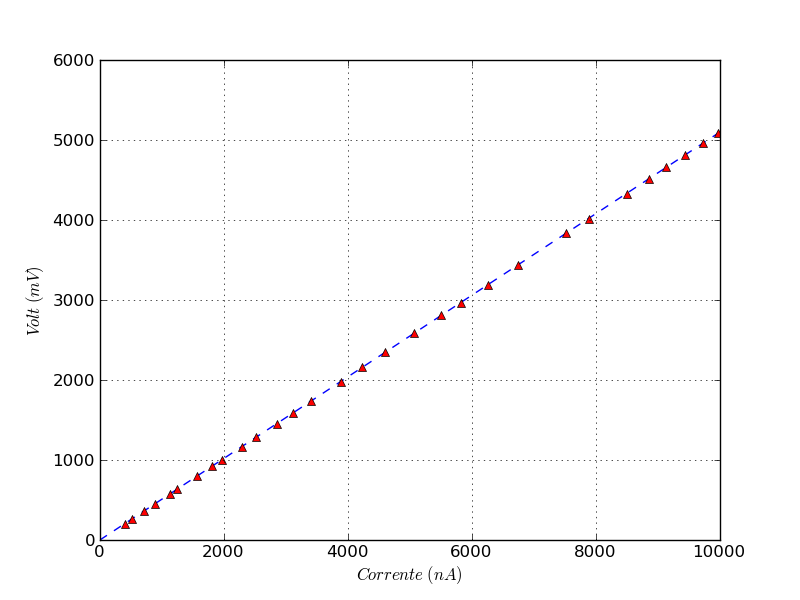
\includegraphics[scale=0.75]{grafici/C1/res1.png}
\

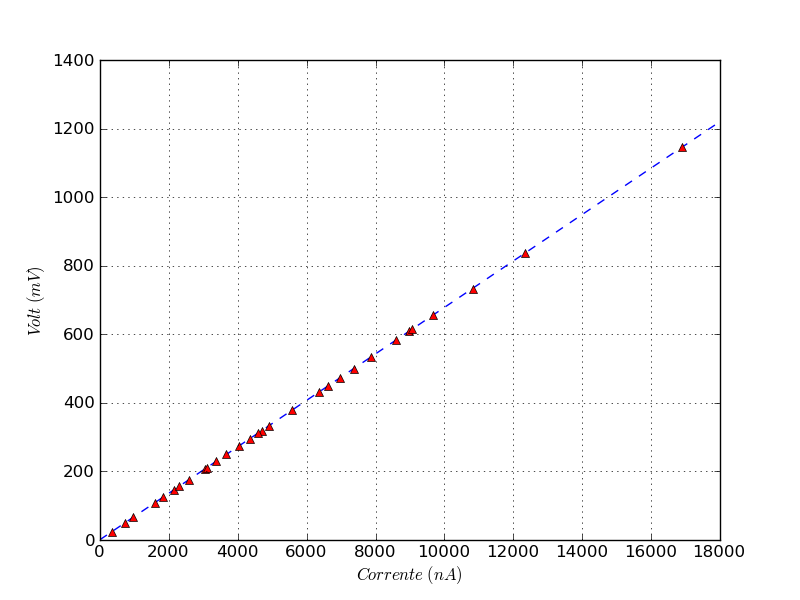
\includegraphics[scale=0.75]{grafici/C1/res2.png}

Misuro la resistenza interna del voltometro, mantenendo costante la ddp a $14.5\ V$ e variando la resistenza all'interno del circuito. 
Il voltmetro è in parallelo al circuito, perciò $R_i$:

$$R_i = \frac{RV}{RI-V} $$

dove R è la resistenza variabile, I la corrente nel circuito e $V= 14.5\ V$

\begin{center}
\begin{tabular}{*{2}{c}}
Resistenza $M\Omega$ & Corrente $nA$
\midline 
7&      36\\
9&      32\\
10& 30\\
11&     29\\
12&     28\\
13&     27\\
14&     26\\
15&     26\\
16&     25\\
17&     24\\

\end{tabular}

La resistenza risulta $9.20 \pm 0.27 \ M \Omega$.


Misuriamo la resistenza interna dell'amperometro, che è collegato in serie al circuito. 

$$R_i = \frac{V-RI}{I}$$

In questo caso, R è fissato ($R=0.5 \Omega$) e sono V e I a variare
\begin{tabular}{*{2}{c}}
Volt $mV$ & Corrente $nA$
\midline
22&      1769\\
40&      3271\\
60&      5047\\
105&     8938\\
133&     11201\\
142&     12021\\
164&     13882\\
174&     14745\\
208&     17604\\
232&     19671\\



\end{tabular}

La resistenza interna risulta $11.42 \pm 0.45 \Omega$


\end{center}


Colleghiamo una piccola lampada a filamento al circuito, e verifichiamo che il suo comportamento resistivo non segue la legge di Ohm. 

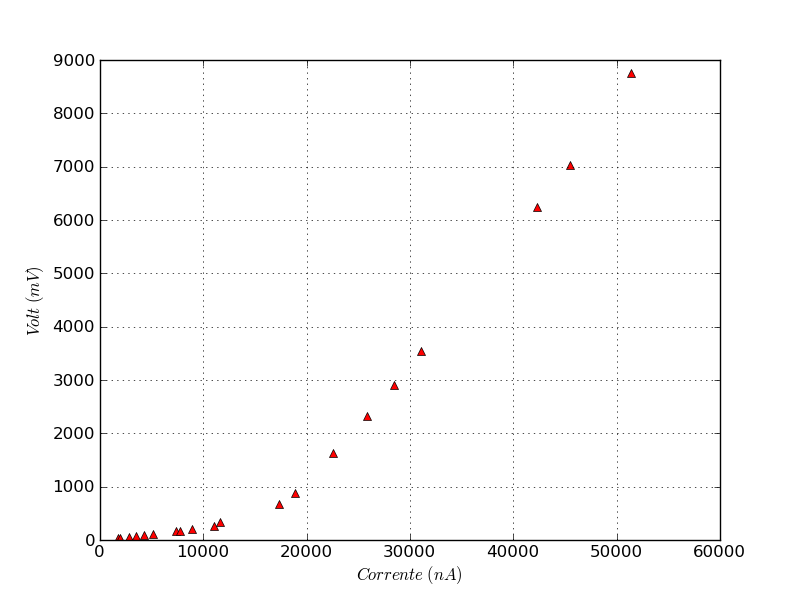
\includegraphics[scale=0.75]{grafici/C1/lampa.png}

La lampadina ha un comportamento non-ohmico nel momento in cui il filamento si scalda sufficientemente e inizia ad emettere luce ($\~500mV$).




